\documentclass[10pt,letterpaper]{article}
\usepackage[top=0.85in,left=2.75in,footskip=0.75in]{geometry}
\usepackage{bibentry}

% Text layout specific to Supplemental Materials
\topmargin 0.0cm
\oddsidemargin 0.5cm
\evensidemargin 0.5cm
\textwidth 16cm
\textheight 21cm

\setlength{\parskip}{1em}

% Template for PLoS
% Version 3.2 March 2016

% General commands for text/figures

% Page margin
\usepackage[top=0.85in,left=2.75in,footskip=0.75in]{geometry}
% Use Unicode characters when possible
\usepackage[utf8x]{inputenc}
% amsmath package, useful for mathematical formulas
\usepackage{amsmath}
%\usepackage{natbib}
% amssymb package, useful for mathematical symbols
\usepackage{amssymb}
%\usepackage{booktabs}
\usepackage{xspace}
\usepackage{hyperref}
% graphicx package, useful for including eps and pdf graphics
% include graphics with the command \includegraphics
\usepackage{graphicx}

% Use adjustwidth environment to exceed column width (see example table in text)
\usepackage{changepage}

% textcomp package and marvosym package for additional characters
\usepackage{textcomp,marvosym}

% fixltx2e package for \textsubscript
\usepackage{fixltx2e}

% cite package, to clean up citations in the main text. Do not remove.
\usepackage{cite}
\usepackage{caption}
\usepackage{subcaption}
\usepackage{rotating}

\usepackage{color}

% Use doublespacing - comment out for single spacing
%\usepackage{setspace}
%\doublespacing


% Bold the 'Figure #' in the caption and separate it with a period
% Captions will be left justified
\usepackage[labelfont=bf,labelsep=period,justification=raggedright]{caption}

% Use the PLoS provided bibtex style
%\bibliographystyle{/Users/stephens/Dropbox/Documents/stylefiles/plos2009}

% Remove brackets from numbering in List of References
\makeatletter
\renewcommand{\@biblabel}[1]{\quad#1.}
\makeatother

% Use nameref to cite supporting information files (see Supporting Information section for more info)
\usepackage{nameref,hyperref}

% line numbers
%\usepackage[right]{lineno}

% ligatures disabled
\usepackage{microtype}
\DisableLigatures[f]{encoding = *, family = * }

% Leave date blank
\date{}

%\pagestyle{myheadings}
%% ** EDIT HERE **
\usepackage{enumerate}
\usepackage{multirow}
\usepackage{url}
\usepackage{xr} %for cross-referencing
%% ** EDIT HERE **
%% PLEASE INCLUDE ALL MACROS BELOW
\newtheorem{algorithm}{Algorithm}
\newtheorem{proposition}{Proposition}
\newtheorem{restateproposition}{Proposition}
\newtheorem{lemma}{Lemma}
\newtheorem{corollary}{Corollary}
\newtheorem{result}{Result}
\newtheorem{note}{Note}
\newtheorem{definition}{Definition}

\def\KL{\text{KL}}

% Text layout
\raggedright
\setlength{\parindent}{0.5cm}
\textwidth 5.25in
\textheight 8.75in

% Bold the 'Figure #' in the caption and separate it from the title/caption with a period
% Captions will be left justified
\usepackage[aboveskip=1pt,labelfont=bf,labelsep=period,justification=raggedright,singlelinecheck=off]{caption}
\renewcommand{\figurename}{Fig}

%------ bibliography
% Use the PLoS provided BiBTeX style
\bibliographystyle{bmc-mathphys}
% Remove brackets from numbering in List of References
\makeatletter
\renewcommand{\@biblabel}[1]{\quad#1.}
\makeatother


%% Author's settings
\def\KL{\text{KL}}

\pagestyle{empty} %%in order to delete the number at the bottom of the page


\begin{document}
\section*{Figures}
\newpage

\begin{figure*}[h!]
\centering
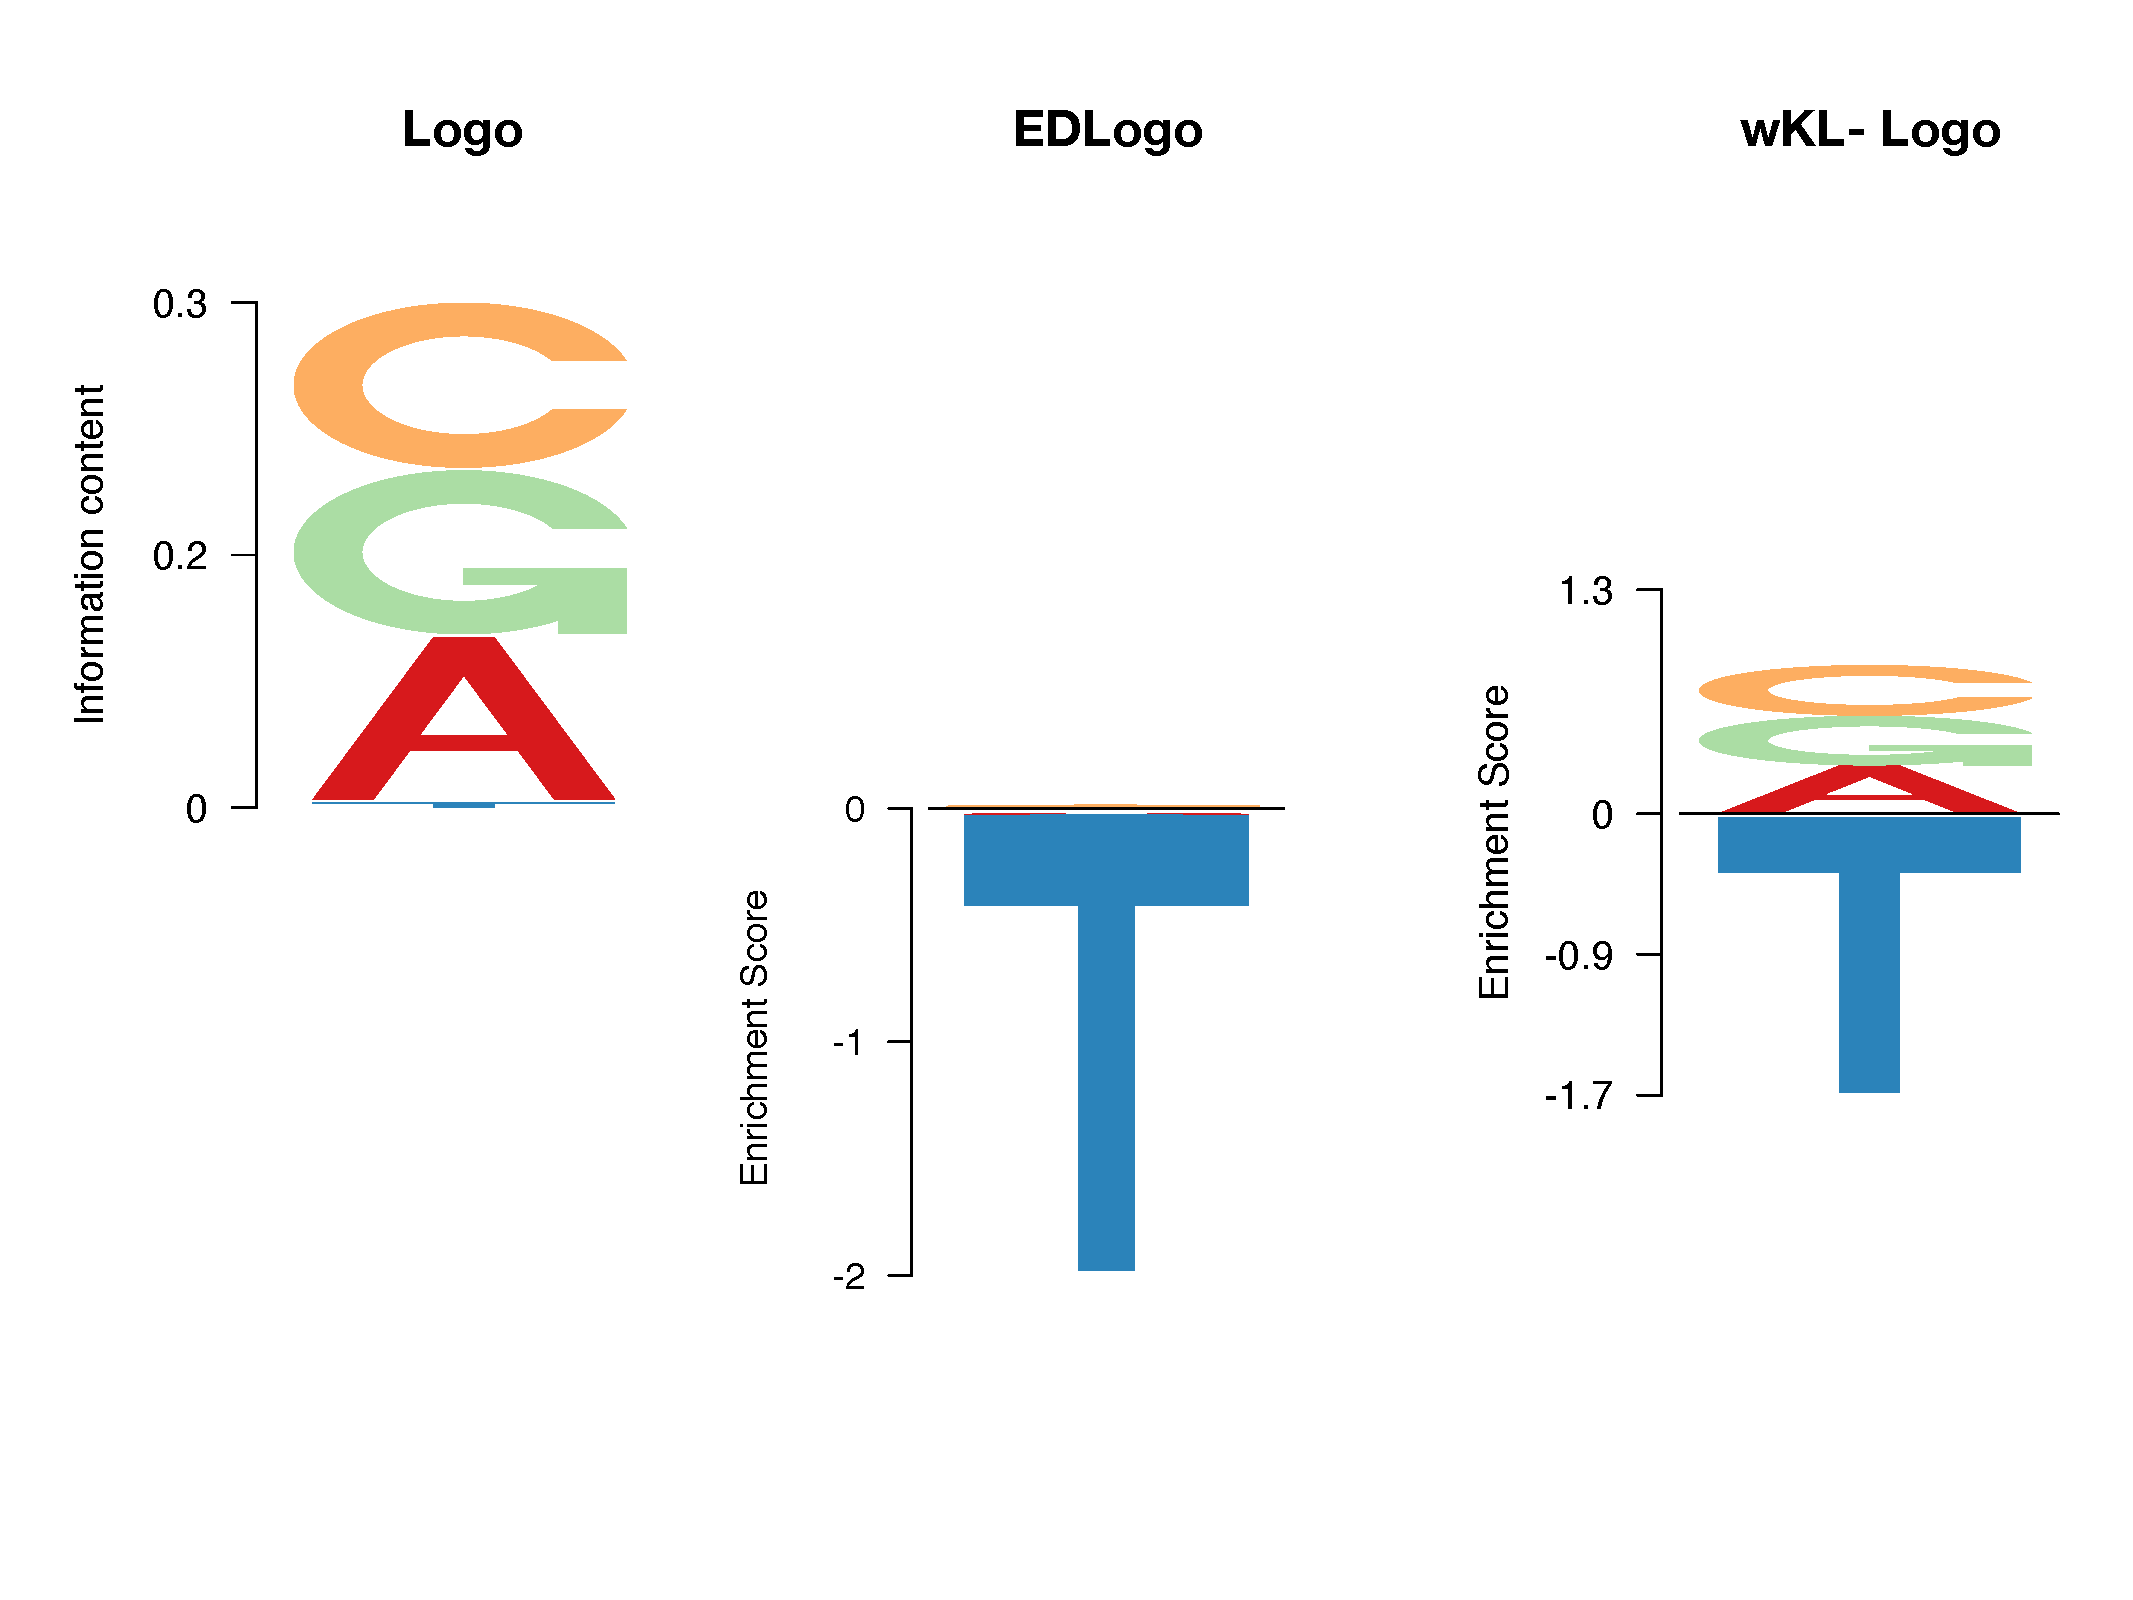
\includegraphics[height=6in, width=7in]{../figures/Figure4/Figure4_2.pdf}
\caption{ \textbf{Comparative illustration of the standard logo, EDLogo and weighted KL logo representations.}
      We present a demo illustration of the standard logo, EDLogo and wKL-Logo for a positional weight vector $p = (p_A, p_C, p_G, p_T) = (0.33, 0.33, 0.33, 0.01)$. Note that the standard logo hightlights the enrichment of A, C and G bases at this position, \textit{EDLogo} highlights the depletion of the base T only, while the weighted KL logo shows both the enrichment of A, C and G as well as the depletion of T at this position.}
\label{fig:fig0}
\end{figure*}

\begin{figure*}[h!]
\centering
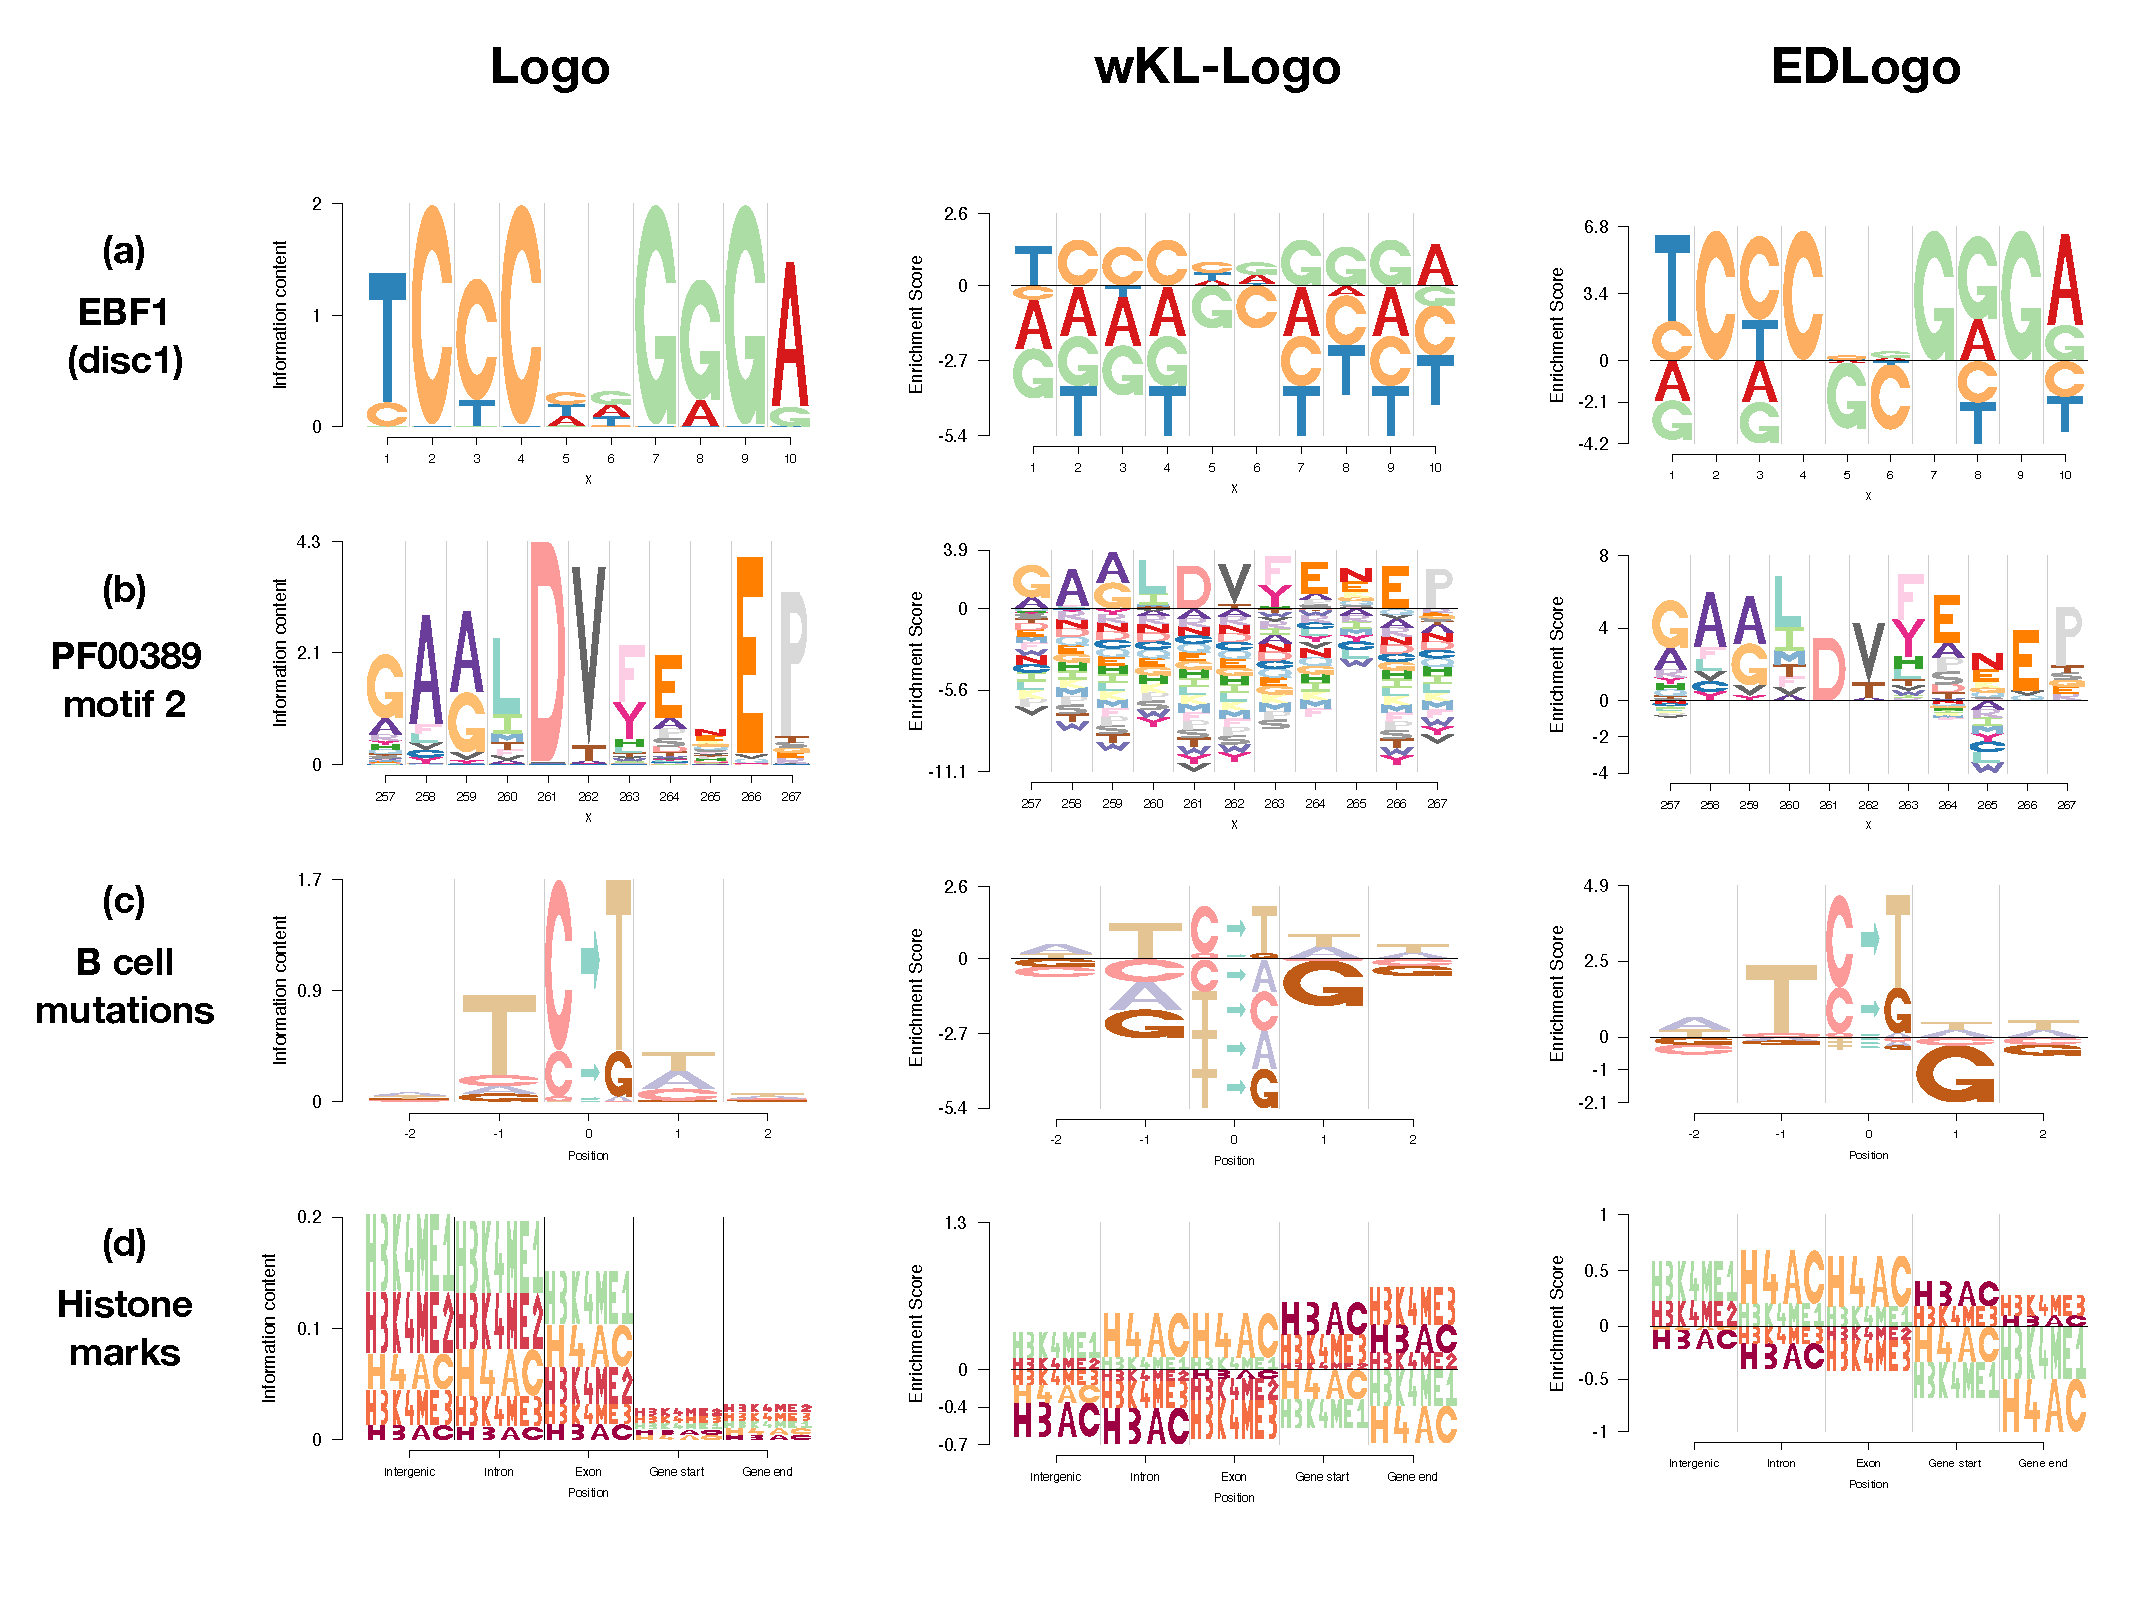
\includegraphics[height=6in, width=7in]{../figures/Figure1/Figure1_3.pdf}
 \caption{\textbf{Comparison of standard logo, weighted KL logo and EDLogo representations for various studies.} 
  In (panel (A)), we present the logo representation of the transcription factor binding site of the EBF1-disc1 transcription factor. \textit{EDLogo} plot captures more clearly the depletion of G and C in the middle of the sequence and the overall palindromic nature of the enrichment and depletion in the binding motif, compared to the other approaches. In panel (B), we compare the three approaches with respect to visualizing the binding motif (Motif2 Start=257 Length=11) of the protein \textit{D-isomer specific 2-hydroxyacid dehydrogenase, catalytic domain (IPR006139)}. We observe that the \textit{EDLogo} representation is visually more parsimonious and detailed than the weighted KL logo. For the plots in panels (C) and (D), we use the string symbols feature of \textit{Logolas}. In panel (C), we present the logo representation of the mutational signature profile of the all mutations in lymphoma B cells, with data taken from Alexandrov et al 2013 \cite{Alexandrov2013}. The depletion of G to the right of the mutation - possibly occurring due to the rarity of CpG sites owing to de-amination of methylated cytosines - is highlighted more clearly in the \textit{EDLogo} representation compared to the other approaches. In panel (D), we present the logo representations of the relative abundance distribution of histone modification sites across various genomic regions in the lymphoblastoid cell line GM06990 (Table S2 in Koch et al 2007 \cite{Koch2007}). The EDLogo representation is more interpretable, in particular at the gene start and gene end regions, compared to the standard logo and reflects patterns in histone marks across various regions along expected lines.}
\label{fig:fig1}
\end{figure*}

\end{document}

